\section{rnode Strukturreferenz}
\label{structrnode}\index{rnode@{rnode}}
{\tt \#include $<$hashtab.h$>$}

Zusammengeh\"{o}rigkeiten von rnode:\begin{figure}[H]
\begin{center}
\leavevmode
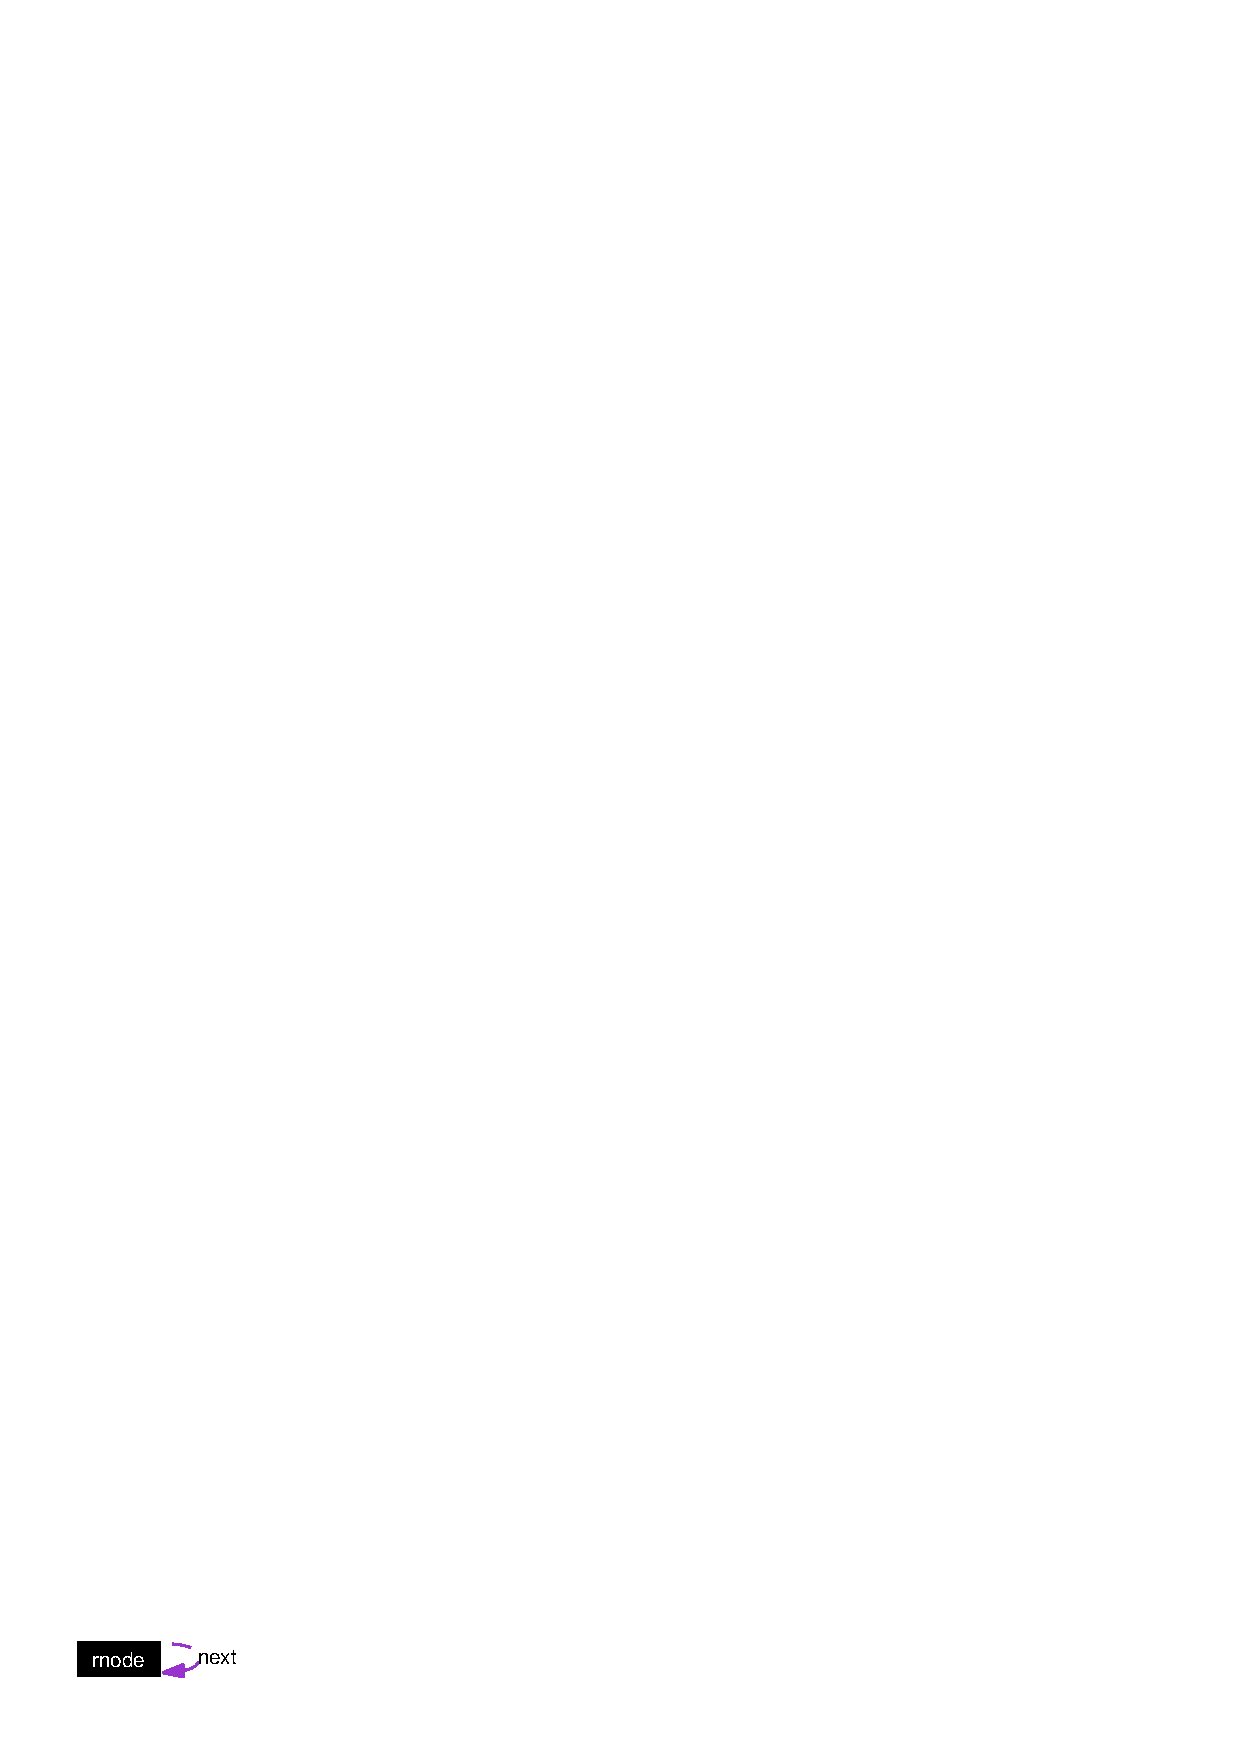
\includegraphics[width=58pt]{structrnode__coll__graph}
\end{center}
\end{figure}
\subsection*{Datenfelder}
\begin{CompactItemize}
\item 
char $\ast$ {\bf string}
\item 
int {\bf flag}
\item 
u\_\-long {\bf count}
\item 
{\bf rnode} $\ast$ {\bf next}
\end{CompactItemize}


\subsection{Ausf\"{u}hrliche Beschreibung}




Definiert in Zeile 45 der Datei hashtab.h.

\subsection{Dokumentation der Datenelemente}
\index{rnode@{rnode}!count@{count}}
\index{count@{count}!rnode@{rnode}}
\subsubsection{\setlength{\rightskip}{0pt plus 5cm}u\_\-long {\bf rnode::count}}\label{structrnode_4034f46036f5fa702a86b3609d7a557a}




Definiert in Zeile 47 der Datei hashtab.h.

Wird benutzt von all\_\-refs\_\-page(), dump\_\-all\_\-refs(), new\_\-rnode(), put\_\-rnode() und top\_\-refs\_\-table().\index{rnode@{rnode}!flag@{flag}}
\index{flag@{flag}!rnode@{rnode}}
\subsubsection{\setlength{\rightskip}{0pt plus 5cm}int {\bf rnode::flag}}\label{structrnode_d5613de994a7efcb74acdb20ac8c2913}




Definiert in Zeile 46 der Datei hashtab.h.

Wird benutzt von all\_\-refs\_\-page(), dump\_\-all\_\-refs(), new\_\-rnode(), put\_\-rnode() und top\_\-refs\_\-table().\index{rnode@{rnode}!next@{next}}
\index{next@{next}!rnode@{rnode}}
\subsubsection{\setlength{\rightskip}{0pt plus 5cm}struct {\bf rnode}$\ast$ {\bf rnode::next}}\label{structrnode_92d155180af669f0207cd3682c132468}




Definiert in Zeile 48 der Datei hashtab.h.

Wird benutzt von del\_\-rlist(), load\_\-ref\_\-array() und put\_\-rnode().\index{rnode@{rnode}!string@{string}}
\index{string@{string}!rnode@{rnode}}
\subsubsection{\setlength{\rightskip}{0pt plus 5cm}char$\ast$ {\bf rnode::string}}\label{structrnode_6709bc4db86e039dd874dede6175a4d1}




Definiert in Zeile 45 der Datei hashtab.h.

Wird benutzt von all\_\-refs\_\-page(), del\_\-rlist(), dump\_\-all\_\-refs(), new\_\-rnode(), put\_\-rnode() und top\_\-refs\_\-table().

Die Dokumentation f\"{u}r diese Struktur wurde erzeugt aufgrund der Datei:\begin{CompactItemize}
\item 
oosalizer/{\bf hashtab.h}\end{CompactItemize}
